\documentclass[10pt, twocolumn]{article}
\usepackage[utf8]{inputenc}
\usepackage[margin=0.75in]{geometry}
\usepackage{setspace}
\usepackage{listings}
\renewcommand\lstlistingname{Algorithm}
\renewcommand\lstlistlistingname{Algorithms}
\lstset{breaklines=true}
\usepackage{hyperref}
\usepackage[pdftex]{graphicx}
\DeclareGraphicsExtensions{.jpg}
\usepackage{amsmath}
\newcommand*{\permcomb}[4][0mu]{{{}^{#3}\mkern#1#2_{#4}}}
\newcommand*{\perm}[1][-3mu]{\permcomb[#1]{P}}
\newcommand*{\comb}[1][-1mu]{\permcomb[#1]{C}}


\title{\vspace{-2.0cm} Beam Search in Comparison to Simulated Annealing as Applied to Job Scheduling}
\author{Connor Hanlon}

\begin{document}
\maketitle

\section{Introduction}

There is a growing necessity for fast, reliable algorithms to solve optimization problems. From speech recognition to job scheduling, these tasks tend to be NP hard in complexity. Therefore it is essential to utilize algorithms that are the most suited for a desired problem, one that balances the tradeoff between space and time complexity, as well as returning an acceptable solution\footnote{An acceptable solution is not necessarily an optimal solution.}. Two algorithms in particular, Simulated Annealing and Beam Search, have been used for optimization problems as they are able to search a solution space with relatively minimal space requirements and much less time in comparison to uninformed search algorithms. The two local search algorithms have been analyzed as applied to a job scheduling problem to determine their efficacy, and the scenarios in which they can be best utilized.

The job scheduling problem which the local search algorithms have been applied to is a simple one. A set of jobs with a corresponding time to complete the job are assigned to a set of people. The goal of this optimization problem is to distribute the jobs among people such that the time to complete all jobs is minimized if all people start their job at the same time. The job scheduling problem is a good problem to study as the size of the solution space is quite large, and uninformed search algorithms quickly become intractable as the number of jobs and number of people increases.


Three experiments were conducted comparing Beam Search and Simulated Annealing as applied to the job scheduling problem. Beam Search consistently produced solution states that were less optimal than Simulated Annealing, however it examined much fewer states and the runtime was much quicker. The Beam Search performed better when the time to search was shorter, however Simulated Annealing outperformed Beam Search over a longer period of time. If speed to find a solution is preferred over optimality of a solution, then Beam Search is the preferred algorithm.


\section{Algorithm Descriptions}

The algorithms Beam Search and Simulated Annealing are both local search algorithms, which search a solution space and apply an objective function to find the most optimal solution. The objective function determines whether a current state has reached the goal state. Local search algorithms are typically not optimal but intrinsically complete as every current state of the search is a solution state.



\subsection{Beam Search}

The Beam Search algorithm is most commonly used with machine translation and speech recognition, but also with planning, job scheduling, among others\cite{alves}. Beam Search only expands the best neighbors as determined by its objective function. It is generally not complete or optimal, which depends on a number of factors, one being the width of the beam of the search\cite{hansen}. The benefit of using the Beam Search lies in the ability to advance through large solution spaces with very little memory consumption.

\begin{lstlisting}[caption={ Beam Search}]
BeamSearch(beam_size, int_node):
    beam = []
    succ = []
    last_nodes = []
    succ_states = createSuccessors(int_node.state, beam_size)
    beam = makeNodes(succ_states)
    While beam not empty:
        for node in beam:
            succ_neighbors = createAllSucc(node, beam_size)
            best_succ = bestSucc(succ_neighbors)
            if best_succ.value == 0:
                return best_succ
            else if best_succ.value <= node.value:
                succ.append(best_succ)
            else:
                last_nodes.append(node)
        beam = succ
        succ = []
    for every node in last_nodes:
        return best node
\end{lstlisting}

The Beam Search algorithm works by selecting multiple solution states, where the number of solution states selected is determined by the beam size of the search, and the selected states form the beam of the search. The search progresses by examining every neighbor state of each state within the beam, and if the neighbor has a more desirable state than the state in the beam, the beam state is replaced with the neighbor. Otherwise if the neighbor is less desirable than the beam state, the beam drops the beam node from the search. The beam therefore decreases by one, and the process is repeated until all states in the beam have been removed or a goal state has been reached. Finally, all dropped beam states are evaluated with each other, and the best of the beam states is returned as the solution. For the pseudocode pertaining to Beam Search, please see Algorithm 1.

% // time and space complexity: breadth = beam, depth = ? , memory = beam
% // gets stuck in local optima

\begin{figure}[!h]
    \centering
    \begin{tabular}[b]{c}
        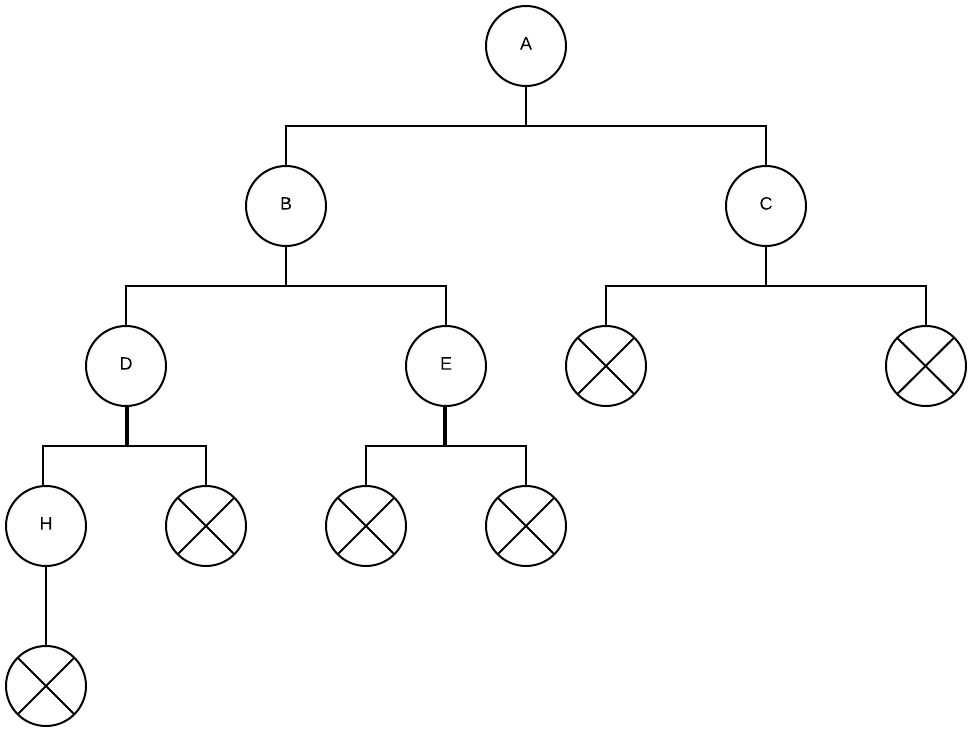
\includegraphics[width=.8\linewidth]{beamsearch.png} \\
    \end{tabular} \qquad
    \caption{Example Beam Search with beam size of 2.}  \label{beam_fig}
\end{figure}

Beam Search is similar to Breadth First Search(BFS) search, where the the states within the beam correspond to the breadth of the BFS search. As shown by Figure \ref{beam_fig}, the breadth of the Beam Search steadily decreases as the search progresses, and only the states within the beam are held in memory which is the biggest difference between BS and BFS.

Due to the similarity of Beam Search to BFS, the worst case time complexity is the same as BFS. If the solution space is infinite and every neighbor selected has a better evaluation than the beam state, then the beam size never decreases. If the beam size is denoted as m and the point at which a single beam state is removed from the beam as d, then the time complexity is O($m^d$). This is the complexity in order to remove a single beam state. The Space complexity of the algorithm is much more appealing than that of BFS, as the only states held in memory are the states within the beam. Therefore, the space complexity is O(m). It is important to note that these complexities are the worst case, due to the fact that Beam Search works solely within the solution space, it is possible to find a solution from the very first state examined.

\subsection{Simulated Annealing}
Simulated annealing is another local search, and provides a good basis to test beam search against as they are of the same classification of search. Simulated Annealing works by generating only one state at each iteration of its search. The objective function is applied to the newly generated state, and if the state is more desirable than the current state of the search, then the search transitions to the newly generated neighbor state. However, if the neighbor state's evaluation is worse than the current state, the algorithm implements a temperature function to determine the next course of action of the search.

In order to avoid getting trapped in a local optima, random moves to states worse than the current state are required. The temperature function determines whether to move to a worse state, and makes the decision to move based on the probability that a move to the worst state is the best action to make. As the search progresses, the probability of a less desirable state to be on the path to the optimal solution decreases. The Simulated Annealing algorithm concludes search when the probability to move is reduced to 0, or the goal state is found.

The space complexity of Simulated Annealing is extremely low, as the current state of the search and the neighbor state are the only states stored in memory at any given moment. Therefore, the space complexity is constant. The worst case time complexity of Simulated Annealing depends on the temperature function, if allowed the search could continue through the solution space indefinitely. Due to the random nature of the search, and the fact that every state examined is within the solution space, the very first state examined has the potential to be the best solution.

\subsection{Beam Search and Simulated Annealing Complexity Analysis}
Local search algorithms are typically flawed, as they tend to be greedy and get stuck within local optima in the solution space. Beam Search suffers from this drawback, therefore the algorithm is not an optimal one. Simulated Annealing, however, utilizes random sideways movements within the solution space to avoid getting stuck within a local optima. The ability to avoid local optima allows for the algorithm to find an optimal solution with probability approaching 1.

Both algorithms are complete, as they search only within the solution space and always guaranteed to return a state from within the solution space.

\subsection{The Objective Function}

The objective function is used to determine the desirability of any given solution state. For every state, the objective function is applied to check whether a solution has been found, and if one it not found, informs the search about the state being evaluated. The search directs its focus based almost entirely on the objective function evaluation. In the case of Simulated Annealing however, the temperature function allow uses the objective function's evaluation to transition to states that are seemingly less desirable.

The objective function utilized for the job scheduling works to minimize the difference between the person with the least amount of job completion time with the person who has the maximum amount of job completion time. The goal is to evenly distribute all jobs such that all people take the same amount of time to complete their assigned jobs, therefore the objective function evaluates to 0 when the goal state is reached.

\subsection{Neighbor Selection Functions}

Due to the fact that Beam Search examines every neighbor to determine the best state to transition to, the approach to neighbor selection greatly affects how the search operates and the time complexity of the search. Simulated Annealing is affected to a lesser extent, as the number of neighbor states examined per iteration is limited to one. Two different neighbor selection functions were utilized by Beam Search and Simulated Annealing in order to exemplify how the neighbor selection affects the two algorithms' search time complexity.

The first neighbor selection function, termed "Combination", was defined as every combination of person per job, regardless of the initial state. The number of neighbors examined is very large, inefficient and quickly becomes intractable as the number of jobs increases. If there are n people assigned to m jobs, the total neighbors selected is $n^m$. The combination selection function was chosen as a basis for comparison to determine how an extremely inefficient neighbor selection function affects both Beam Search and Simulated Annealing.

The second neighbor selection function defined a neighbor as a variation of the original state, in which the person with the maximum job completion time is replaced with other people of lesser job completion times. The "max" neighbor selection function limits the amount of neighbors generated to the the number of people available to replace one of the jobs assigned to the person with max job completion time. If the the total number of people available for a given job is n, then the number of neighbors selected is n. The max neighbor selection is a relatively efficient selection function in comparison to the combination selection function, and provides for a good basis of comparison for the local search algorithms.


\section{Experimental Methodology}

% /// changed runtime limits for search with experiment 2 because when the beam increases, more nodes must be examined and to determine the actual efficacy of the algorithm, the time constraint had to be relaxed

Each experiment configuration was conducted using 5 trials. Multiple iterations provides for an accurate measurement of time, and minimizes the affect of external processes on the search results. The number of people was held constant at 4, and the amount of time allocated per trial was limited to 5 minutes. Once the search reached the 5 minute limit, the best, current state of the search was returned.

The runtime of each trial was measured by starting a timer at the instant a search began, and ended when the search found a desirable solution. In order to reduce any external processes from affecting the results of the experimental trials, the states of the search was tracked and recorded. The tracking of states was done by creating nodes that contained current state information. The time required to generate a node during a search is constant, therefore keeping track of the total node count is an effective way to determine the runtime of a search without explicitly measuring time.

Three different types of experiments were conducted. Experiment one examined how the Beam Search handles larger problem sizes, and compared it to the flexibility of the Simulated Annealing algorithm to do the same. Five different job scheduling problem sizes were experimented with, setting the number of jobs to 6 through 10, incrementing by 1 per problem size increase. The reason for holding the number of jobs relatively low is due to the exponentially increasing complexity of neighbor selection at higher problem sizes, which results in larger space and time requirements beyond the ability to properly experiment with.

The second experiment type varied the neighbor selection function used by both the Beam Search and Simulated Annealing. Beam search works by examining all successor's neighbors, and depending on the neighbor selection the number of neighbors examined has the potential to being quiet large. Two neighbor selection functions were used, one which defined a neighbor in such a way that limited the amount of neighbors selected for comparison, and another which defined a neighbor that compared a much larger amount of neighbors selected for comparison in contrast to the first neighbor selecting function.

The third experiment varied the size of the beam of the beam search. Five beam sizes were used, with a beam size of 5 through 25 and incrementing beam size by 5 per iteration. The intent was to determine at which beam size the algorithm is most effective, and whether the most effective beam size for Beam Search is more effective than Simulated Annealing.

\section{Experimental Results and Analysis}

In this section, the experimental results comparing Beam Search with Simulated Annealing is presented. Both algorithms were implemented in Python 3.7.0, and used the same job scheduling implementation, neighbor selection functions, objective functions, and data collection process. The experimental results are broken down and analyzed in three separate sections as follows: Problem Size, Beam Size, and Neighbor Function. In the fourth and final subsection, Beam Search and Simulated Annealing are directly compared using the results of all experiments in conjunction with each other.

\subsection{Problem Size}

Beam search and Simulated Annealing were relatively time consistent in respect to the size of the problem and solution space they traversed. Graphs from Figure \ref{exp_one}(a) and Figure \ref{exp_one}(b) indicate that the runtime and total node count stay consistent as the amount of jobs increase for both BS and SA, which corroborates the conclusion that the time to complete search remained constant. This is explained easily by the method by which both local algorithms search a solution space and the self directing nature of the algorithms.

\begin{figure}[!h]
    \centering
    \begin{tabular}[b]{c}
        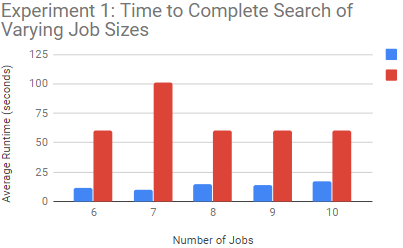
\includegraphics[width=.90\linewidth]{exp_one_time.png} \\
        \small (a)
    \end{tabular} \qquad
    \begin{tabular}[b]{c}
        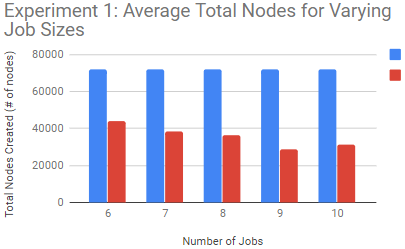
\includegraphics[width=.90\linewidth]{exp_one_nodes.png} \\
        \small (b)
    \end{tabular}
     \begin{tabular}[b]{c}
        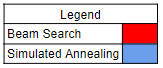
\includegraphics[width=.3\linewidth]{legend.png} \\
        \small Legend for Figure \ref{exp_one}
    \end{tabular}
    \caption{Average runtimes \ref{exp_one}(a) and average node count \ref{exp_one}(b) for varying job amounts for BS and SA.}  \label{exp_one}
\end{figure}


The search algorithms are also consistent in the average objective function evaluation upon completion of search as shown in Figure \ref{exp_one_obj}. This indicates that both algorithms can scale efficiently to problem sizes with large solution spaces and consistently produce results relatively close to a range of predictable solutions.

\begin{figure}[!h]
    \centering
    \begin{tabular}[b]{c}
        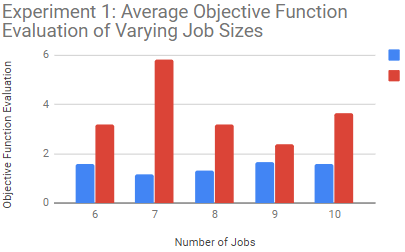
\includegraphics[width=.90\linewidth]{exp_one_obj.png} \\
    \end{tabular} \qquad
     \begin{tabular}[b]{c}
        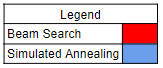
\includegraphics[width=.3\linewidth]{legend.png} \\
        \small Legend for Figure \ref{exp_one_obj}
    \end{tabular}
    \caption{Average objective function evaluation for varying job amounts for BS and SA.}  \label{exp_one_obj}
\end{figure}


\subsection{Neighbor Selection}

The neighbor selection had a significant impact on the efficiency of both algorithms. In terms of average runtime, the Max neighbor selection function outperformed the Combination neighbor selection function by completing search twice as fast\footnote{Twice as fast signifies that the runtime for the Max selection search was half that of the Combination selection search} for Beam Search
and roughly 25\% faster\footnote{25\% faster signifies that the runtime for the Max selection search was 75\% of the runtime of the Combination selection search.} for Simulated Annealing according to Figure \ref{exp_three}.

\begin{figure}[!h]
    \centering
    \begin{tabular}[b]{c}
        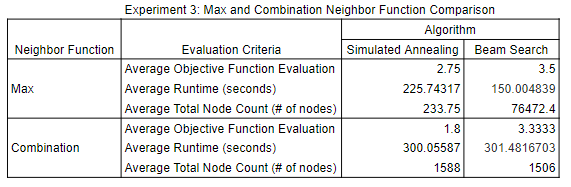
\includegraphics[width=1\linewidth]{exp_three.png} \\
    \end{tabular} \qquad
    \caption{Comparison of Max and Combination Neighbor Selection Functions with Beam Search and Simulated Annealing.}  \label{exp_three}
\end{figure}

Total node count was significantly higher for the Max neighbor selection function in comparison with the Combination selection function for Beam Search as shown by Figure \ref{exp_three}. The reason for this is easy to explain: the Max function selects much fewer states than Combination selection. If the number of people available for job assignment is n and the total amount of jobs is m, then the time complexity of Combination is O($n^m$), whereas Max is O(n). Nodes are created after all neighbor states are selected, therefore Max generated significantly more nodes because less time was consumed in the initial selection of states.

% As for Simulated Annealing, the total node count is lower with the use of Max than with Combination as indicated by Figure \ref{exp_three}. The reason for this is due to the **

The Combination neighbor selector outperformed the Max selector in one aspect, as the average objective function value decreased for both Simulated Annealing and Beam Search as indicated by Figure \ref{exp_three}. The Combination selector extends the search to a much larger solution space, whereas the Max selector chooses a much smaller set of states from the solution space. Therefore, the algorithms utilizing Max must search for a longer period of time and examine more states in order to decrease the objective function evaluation.


\subsection{Beam Size}

As the size of the beam increased for Beam Search, Figure \ref{exp_two} indicates that the number of nodes examined increased by an average of 1,236 nodes at each new beam size. It is linear in nature according to the preliminary data obtained, however with further experimentation using larger problem sizes, more time to conduct the experiments, and beam size, a more accurate description of the rate of node increase can be determined.

\begin{figure}[!h]
    \centering
    \begin{tabular}[b]{c}
        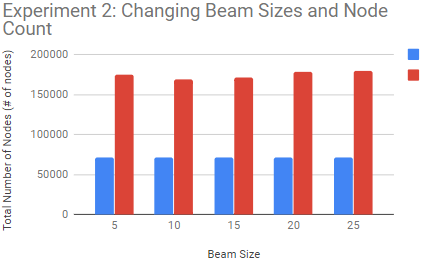
\includegraphics[width=.70\linewidth]{exp_two_node.png} \\
        \small (a)
    \end{tabular} \qquad
    \begin{tabular}[b]{c}
        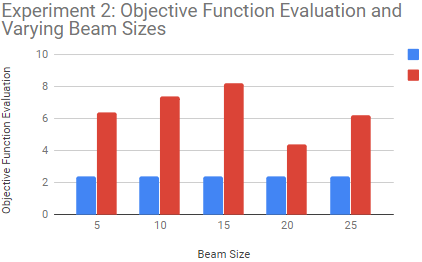
\includegraphics[width=.70\linewidth]{exp_two_obj.png} \\
        \small (b)
    \end{tabular}
     \begin{tabular}[b]{c}
        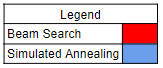
\includegraphics[width=.3\linewidth]{legend.png} \\
        \small Legend for Figure \ref{exp_two}
    \end{tabular}
    \caption{Average node count \ref{exp_two}(a) and average objective function evaluations \ref{exp_two}(b) for varying Beam Sizes for BS in comparison to the standard SA search.}  \label{exp_two}
\end{figure}

For Simulated Annealing, the algorithm was held constant for all changes in beam size, therefore the total node count remained fixed. The node count was limited by the temperature function, which is the reason for the plateau.


\subsection{Beam Search and Simulated Annealing Comparison}

Simulated Annealing in almost every experiment performed better than Beam Search. When allowed to run to completion without a time limitation, its runtime was shorter on average in comparison to Beam Search. Additionally, Simulated Annealing returned solutions that were more desirable according to the objective function evaluation of the returned solution's state.

Interestingly however, the total nodes created by Simulated Annealing was significantly larger than the Beam Search as shown in Figure \ref{exp_one}. The total node count metric was determined to give an accurate representation of constant runtime, to minimize the affects of external processes on the results of the real-time runtime measurements. The reason for the seemingly contradictory evidence provided by the preliminary data lies in the neighbor selection functions. Both Simulated Annealing and Beam Search utilized the same neighbor selection function, however Simulated Annealing at each iteration only created one node and made one call to the selector function. In contrast, Beam Search called the selector function for every node within the beam, which limited the total amount of nodes that could be generated but also increased the amount of states examined. By casting the search wider, Beam Search increased the time required to find the best solution while also minimizing the amount of nodes required to search for the solution.

\section{Conclusion and Further Work}

The local search algorithms Beam Search and Simulated Annealing have their own strengths and weaknesses while searching solution spaces. Beam Search is effective when there is leniency for the solution returned from the search, and time is prioritized. Beam Search is able to examine multiple states in a shorter time-span than Simulated Annealing, but the solution found is not guaranteed to be the best as BS is a greedy algorithm which is able to get stuck in local optima.

If time is not prioritized and the solution is required to be the most desirable, Simulated Annealing is the most effective algorithm. It is guaranteed to find an optimal solution given enough time to complete the search. This was exemplified in the experiments, where the average objective function values of Simulated Annealing in comparison to Beam Search were significantly lower when the algorithms were given sufficient time to complete the search.

Further analysis of Beam Search and the methods by which to increase the efficiency of the search is conceivable. The search can improve in efficiency by adjusting how neighbors are defined and selected during search. According to the preliminary data within this study, the size of the beam can have negligible effects on the desirability of the solution found, at the expense of time to conduct search.

\begin{thebibliography}{10}

\bibitem{alves} Alves, Rui. ``Beam search algorithms for the early/tardy scheduling problem with release dates,'' {\em Faculdade de Economia da Universidade do Porto}, 2004.

\bibitem{bayiz} Bayiz, Murat. ``Job shop scheduling with beam search,'' {\em European Journal of Operational Research}, pp. 390-412, 1998.

\bibitem{hansen} Hansen, Eric. ``Beam-Stack Search: Integrating Backtracking with Beam Search,'' {\em 15th International Conference on Automated Planning and Scheduling}, 2005.

\bibitem{montoya-torres} Montoya-Torres, Jairo. ``A beam search heuristic for scheduling a single machine with release dates and sequence dependent setup times to minimize the makespan,'' {\em Computers \& Operations Research}, pp. 132-140, 2016.

\bibitem{ting} Ting, Ching-Jung. ``A Beam Search Heuristic for the Traveling Salesman Problem with Time Windows,'' {\em Journal of the Eastern Asia Society for Transportation Studies}, vol. 9, pp. 702-712, 2011.


\end{thebibliography}
\end{document}
